
% v2-acmsmall-sample.tex, dated March 6 2012
% This is a sample file for ACM small trim journals
%
% Compilation using 'acmsmall.cls' - version 1.3 (March 2012), Aptara Inc.
% (c) 2010 Association for Computing Machinery (ACM)
%
% Questions/Suggestions/Feedback should be addressed to => "acmtexsupport@aptaracorp.com".
% Users can also go through the FAQs available on the journal's submission webpage.
%
% Steps to compile: latex, bibtex, latex latex
%
% For tracking purposes => this is v1.3 - March 2012
\documentclass[prodmode,acmtecs]{acmsmall} % Aptara syntax
\usepackage[spanish,polish]{babel}
\usepackage[T1]{fontenc}
\usepackage{fancyvrb}
\usepackage{graphicx,hyperref}
\newcommand\cutout[1]{}


\usepackage[table]{xcolor}
\usepackage[utf8]{inputenc}
\usepackage[parfill]{parskip}
\usepackage{tabulary}
\PassOptionsToPackage{hyphens}{url}
\usepackage{hyperref}    
\usepackage[capitalize]{cleveref}


% Metadata Information
% !!! TODO: SET THESE VALUES !!!
\acmVolume{0}
\acmNumber{0}
\acmArticle{CFP}
\acmYear{0}
\acmMonth{0}

\newcounter{colstart}
\setcounter{page}{4}

\RecustomVerbatimCommand{\VerbatimInput}{VerbatimInput}%
{
%fontsize=\footnotesize,
fontfamily=\rmdefault
}


\newcommand{\UnderscoreCommands}{%\do\verbatiminput%
\do\citeNP \do\citeA \do\citeANP \do\citeN \do\shortcite%
\do\shortciteNP \do\shortciteA \do\shortciteANP \do\shortciteN%
\do\citeyear \do\citeyearNP%
}

\usepackage[strings]{underscore}



% Document starts
\begin{document}


\setcounter{colstart}{\thepage}

\acmArticle{CFP}
\title{{\huge\sc SIGLOG Monthly 233}

 January 2023}
\author{DAVID PURSER\affil{University of Liverpool, UK}
\vspace*{-2.6cm}\begin{flushright}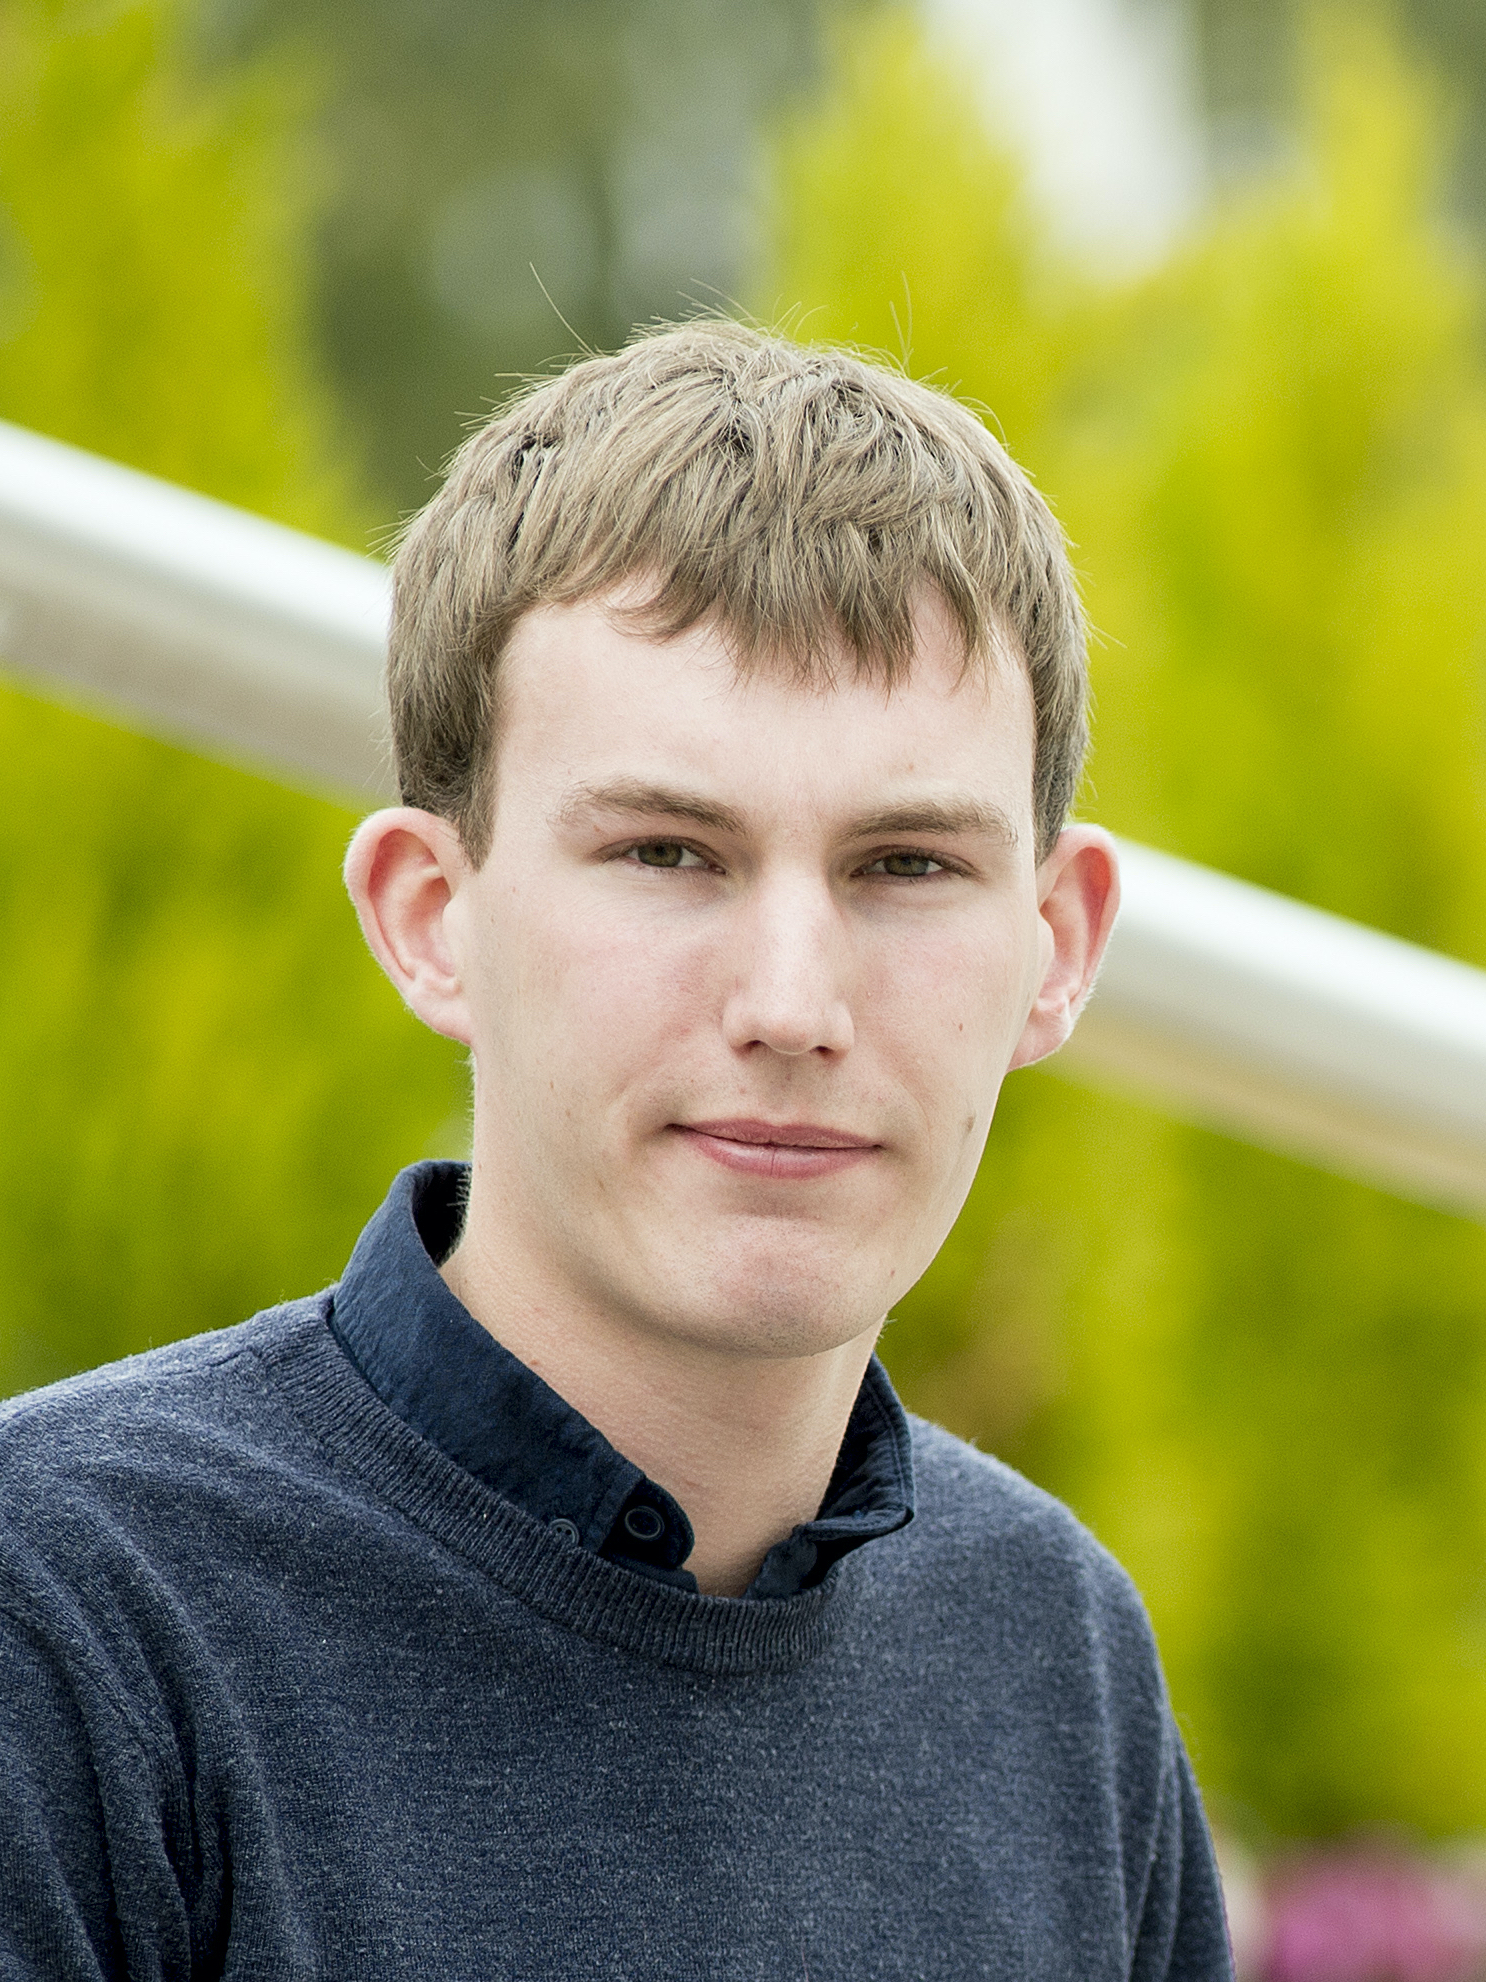
\includegraphics[width=30mm]{dp}\end{flushright}
}

\maketitlee

\href{https://lics.siglog.org/newsletters/}{Past Issues}
 - 
\href{https://lics.siglog.org/newsletters/inst.html}{How to submit an announcement}
\section{Table of Content}\begin{itemize}\item DEADLINES (\cref{deadlines}) 
 
\item SIGLOG MATTERS 
 
\begin{itemize}\item Alonzo Church Award 2023 (\cref{AlonzoChurchAward2023})
\end{itemize} 
\item CALLS 
 
\begin{itemize}\item CPP 2023 (CALL FOR PARTICIPATION) (\cref{CPP2023})
\item CAV 2023 (CALL FOR PAPERS, CALL FOR NOMINATIONS) (\cref{CAV2023})
\item Salomaa Prize (CALL FOR NOMINATIONS) (\cref{SalomaaPrize})
\item ICGT 2023 (CALL FOR PAPERS) (\cref{ICGT2023})
\item FORMATS 2023 (CALL FOR PAPERS) (\cref{FORMATS2023})
\end{itemize} 
\item JOB ANNOUNCEMENTS 
 
\begin{itemize}\item POST-DOC POSITION IN LOGIC at LUCI-UNIMI (\cref{POSTDOCPOSITIONINLOGICatLUCIUNIMI})
\item POSTDOC POSITION in WARSAW (\cref{POSTDOCPOSITIONinWARSAW})
\end{itemize} 
\end{itemize}\section{Deadlines}\label{deadlines}\rowcolors{1}{white}{gray!25}\begin{tabulary}{\linewidth}{LL}LICS 2023:  & Jan 18, 2023 (Titles and Short Abstracts Due), Jan 23, 2023 (Full Papers Due) \\
POST-DOC POSITION IN LOGIC at LUCI-UNIMI:  & Jan 18, 2023 23:59 CET (Applications) \\
ICLP 2023:  & Jan 23, 2023 (Abstract registration), Jan 31, 2023 (Paper (regular, applications, thematic tracks)), Apr 28, 2023 (Paper (other paper types)) \\
FSCD 2023:  & Jan 30, 2023 (Abstract), Feb 03, 2023 (Paper) \\
Dov Gabbay Prize for Logic and Foundations:  & Jan 31, 2023 (Deadline for nominations) \\
S. Barry Cooper Prize:  & Jan 31, 2023 (Deadline for nominations) \\
Alonzo Church Award 2023:  & Feb 01, 2023 (Deadline for nominations) \\
CONFEST 2023:  & Feb 02, 2023 (Submission deadline) \\
CAV 2023:  & Feb 03, 2023 (Paper), Apr 25, 2023 (Artifact), Feb 20, 2023 (CAV AWARD Nomination deadline) \\
CiE 2023:  & Feb 08, 2023 (Abstract), Feb 15, 2023 (Article) \\
ICALP 2023:  & Feb 11, 2023 at 11am CET (Paper) \\
POSTDOC POSITION in WARSAW:  & Feb 15, 2023 (Applications) \\
Salomaa Prize:  & Feb 28, 2023 (Deadline for nominations) \\
ICGT 2023:  & Feb 28, 2023 (Abstract), Mar 07, 2023 (Paper) \\
LOGIC COLLOQUIUM 2023:  & Mar 01, 2023 (Abstract), Mar 01, 2023 (Student Travel Grants deadline) \\
FORMATS 2023:  & Apr 21, 2023 (Abstract), Apr 28, 2023 (Paper) \\
\end{tabulary}
\section{Alonzo Church Award 2023: The 2023 Alonzo Church Award for Outstanding Contributions to Logic and Computation}\label{AlonzoChurchAward2023}CALL FOR NOMINATIONS 

\begin{itemize}\item  INTRODUCTION 
 
  An annual award, called the Alonzo Church Award for Outstanding Contributions to Logic and Computation, was established in 2015 by the ACM Special Interest Group for Logic and Computation (SIGLOG), the European Association for Theoretical Computer Science (EATCS), the European Association for Computer Science Logic (EACSL), and the Kurt Goedel Society (KGS). The award is for an outstanding contribution represented by a paper or by a small group of papers published within the past 25 years. This time span allows the lasting impact and depth of the contribution to have been established. The award can be given to an individual, or to a group of individuals who have collaborated on the research. For the rules governing this award, see \href{https://siglog.org/alonzo-church-award/}{https://siglog.org/alonzo-church-award/}, \href{https://www.eatcs.org/index.php/church-award/}{https://www.eatcs.org/index.php/church-award/}, and \href{https://www.eacsl.org/alonzo-church-award/}{https://www.eacsl.org/alonzo-church-award/}. 
 
  The 2022 Alonzo Church Award was given to Dexter Kozen for his ground- breaking work on the theory and applications of Kleene Algebra with Tests. Lists containing this and all previous winners can be found through the links above.  
 
\item  ELIGIBILITY AND NOMINATIONS 
 
  The contribution must have appeared in a paper or papers published within the past 25 years. Thus, for the 2023 award, the cut-off date is January 1, 1998. When a paper has appeared in a conference and then in a journal, the date of the journal publication will determine the cut-off date. In addition, the contribution must not yet have received recognition via a major award, such as the Turing Award, the Kanellakis Award, or the Goedel Prize. (The nominee(s) may have received such awards for other contributions.) While the contribution can consist of conference or journal papers, journal papers will be given a preference. 
 
  Nominations for the 2023 award are now being solicited. The nominating letter must summarise the contribution and make the case that it is fundamental and outstanding. The nominating letter can have multiple co-signers. Self-nominations are excluded. Nominations must include: a proposed citation (up to 25 words); a succinct (100-250 words) description of the contribution; and a detailed statement (not exceeding four pages) to justify the nomination. Nominations may also be accompanied by supporting letters and other evidence of worthiness. Nominations for the 2023 award are automatically considered for all future editions of the award, until they receive the award or the nominated papers are no longer eligible. Nominations should be submitted to dezani@di.unito.it and to mariangiola.dezani@gmail.com. 
 
Deadline for nominations: Feb 01, 2023 
 
\item  PRESENTATION OF THE AWARD 
 
  The 2023 award will be presented at the 50th EATCS International Colloquium on Automata, Languages and Programming, which is scheduled to take place in Paderborn - Germany on July 10-14, 2023. The award will be accompanied by an invited lecture by the award winner, or by one of the award winners. The awardee(s) will receive a certificate and a cash prize of USD 2,000. If there are multiple awardees, this amount will be shared.  
 
\item  AWARD COMMITTEE 
 
  The 2023 Alonzo Church Award Committee consists of the following five members: Thomas Colcombet, Mariangiola Dezani (chair), Marcelo Fiore, Radha Jagadeesan, and Igor Walukiewicz. 
 
\end{itemize}\section{CPP 2023: Certified Programs and Proofs}\label{CPP2023}  Jan 16-17, 2023, co-located with POPL 2023, Boston\\ 
  Registration: \href{https://popl23.sigplan.org/attending/registration}{https://popl23.sigplan.org/attending/registration}\\ 
  Accommodation: Boston Park Plaza \href{https://popl23.sigplan.org/venue/POPL-2023-venue}{https://popl23.sigplan.org/venue/POPL-2023-venue}\\ 
CALL FOR PARTICIPATION 

\begin{itemize}\item  ABOUT 
 
  Certified Programs and Proofs (CPP) is an international conference on practical and theoretical topics in all areas that consider formal verification and certification as an essential paradigm for their work. CPP spans areas of computer science, mathematics, logic, and education. 
 
  CPP 2023 (\href{https://popl23.sigplan.org/home/CPP-2023}{https://popl23.sigplan.org/home/CPP-2023}) will be held on 16-17 January 2023 and will be co-located with POPL 2023. CPP 2023 is sponsored by ACM SIGPLAN, in cooperation with ACM SIGLOG, and supported by a diverse set of industrial sponsors. Similarly to other events collocated with POPL 2023, CPP will take place as an in-person event at Boston Park Plaza, and will require attendees to provide proof of vaccination (details will be available soon). Virtual participation via Airmeet will also be available; look for updated information about that option on the POPL web site. 
 
  For more information about this edition and the CPP series, please visit \href{https://popl23.sigplan.org/home/CPP-2023}{https://popl23.sigplan.org/home/CPP-2023}  
 
\item  INVITED SPEAKERS 
 
\begin{itemize}\item  Sandrine Blazy, University of Rennes and IRISA
\item  Cezary Kaliszyk, University of Innsbruck
\end{itemize} 
\item  ACCEPTED PAPERS 
 
  The list of accepted papers is available at \href{https://popl23.sigplan.org/home/CPP-2023#event-overview}{https://popl23.sigplan.org/home/CPP-2023\#event-overview} 
 
\end{itemize}\section{CAV 2023: 35th International Conference on Computer-Aided Verification}\label{CAV2023}  July 17-22, 2023, Paris, France\\ 
  \href{http://www.i-cav.org/2023/}{http://www.i-cav.org/2023/}\\ 
CALL FOR PAPERS 

\begin{itemize}\item  CAV 2023 is the 35th in a series dedicated to the advancement of the theory and practice of computer-aided formal analysis methods for hardware and   software systems. The conference covers the spectrum from theoretical results to concrete applications, with an emphasis on practical verification tools and the algorithms and techniques that are needed for their implementation. CAV considers it vital to continue spurring advances in hardware and software verification while expanding to new domains such as machine learning, autonomous systems, and computer security. The proceedings of the conference will be published in the Springer-Verlag Lecture Notes in Computer Science series. 
 
\item  IMPORTANT DATES: (firm) 
 
\rowcolors{1}{white}{gray!25}\begin{tabulary}{\linewidth}{LL}Paper submission:  & Feb 03, 2023 \\
Rebuttal period:  & March 29-31, 2023 \\
Artifact submission:  & Apr 25, 2023 \\
\end{tabulary}
 
\item  Detailed information can be found on the webpage. 
 
\end{itemize}CALL FOR NOMINATIONS 

\begin{itemize}\item CAV AWARD 
 
  The CAV award is given annually at the CAV conference for fundamental contributions to the field of Computer-Aided Verification. 
 
CAV AWARD Nomination deadline: Feb 20, 2023 
 
\end{itemize}\section{Salomaa Prize: Salomaa Prize in Automata Theory, Formal Languages, and Related Topics}\label{SalomaaPrize}  Deadline Feb 28, 2023\\ 
  \href{https://math.utu.fi/salomaaprize/}{https://math.utu.fi/salomaaprize/}\\ 
CALL FOR NOMINATIONS 

\begin{itemize}\item  ABOUT  
 
  The Salomaa Prize in Automata Theory, Formal Languages, and Related Topics is awarded annually at the conference DLT (Developments in Language Theory). It consists of the diploma and the prize of 2000 Euros donated by the University of Turku. The award is given to a distinguished researcher on his/her fundamental achievements on automata theory and related topics. The achievement might be a single article, a series of articles, or a broader impact on the theory. The Salomaa Prize 2023 will be awarded at DLT 2023 In Umea, Sweden. Nominations should be sent to the chair of the selection committee (Wolfgang Thomas, RWTH Aachen University, thomas@cs.rwth-aachen.de). For all further information see the Salomaa Prize website mentioned above.  
 
Deadline for nominations: Feb 28, 2023 
 
\end{itemize}\section{ICGT 2023: 16th International Conference on Graph Transformation}\label{ICGT2023}  \href{https://conf.researchr.org/home/icgt-2023}{https://conf.researchr.org/home/icgt-2023}\\ 
  Part of STAF 2023, 17-21st July in Leicester, UK\\ 
  \href{https://conf.researchr.org/home/staf-2023}{https://conf.researchr.org/home/staf-2023}\\ 
CALL FOR PAPERS 

\begin{itemize}\item  AIMS AND SCOPE  
 
  The use of graphs and graph-like structures as a formalism for specification and modelling is widespread in all areas of computer science as well as in many fields of computational research and engineering. Relevant examples include software architectures, pointer structures, state space and control/data flow graphs, UML and other domain-specific models, network layouts, topologies of cyber-physical environments, quantum computing and molecular structures. Often, these graphs undergo dynamic change, ranging from reconfiguration and evolution to various kinds of behaviour, all of which may be captured by rule-based graph manipulation. Thus, graphs and graph transformation form a fundamental universal modelling paradigm that serves as a means for formal reasoning and analysis, ranging from the verification of certain properties of interest to the discovery of fundamentally new insights. 
 
  The International Conference on Graph Transformation aims at fostering exchange and collaboration of researchers from different backgrounds working with graphs and graph transformation, either in contributing to their theoretical foundations or by applying established formalisms to classical or novel areas. The conference not only serves as a well-established scientific publication outlet, but also as a platform to boost inter- and intra-disciplinary research and to leeway for new ideas. 
 
  The 16th International Conference on Graph Transformation (ICGT 2023) will be held in Leicester, UK, as part of STAF 2023 (Software Technologies: Applications and Foundations). The conference takes place under the auspices of EATCS and IFIP WG 1.3. Proceedings will be published by Springer in the Lecture Notes in Computer Science (LNCS) series. 
 
\item  IMPORTANT DATES (AoE) 
 
\rowcolors{1}{white}{gray!25}\begin{tabulary}{\linewidth}{LL}Abstract submission:  & Feb 28, 2023 \\
Paper submission:  & Mar 07, 2023 \\
Notification:  & Apr 21, 2023 \\
Final version due:  & May 07, 2023 \\
Conference:  & within  Jul 17-21, 2023 \\
\end{tabulary}
 
\item  TOPICS   
 
  In order to foster a lively exchange of perspectives on the subject of the conference, the programme committee of ICGT 2023 encourages all kinds of contributions related to graphs and graph transformation, either from a theoretical point of view or a practical one. 
 
 Topics of interest include, but are not limited to the following subjects: 
 
\begin{itemize}\item  General models of graph transformation (e.g. adhesive categories and hyperedge replacement systems)
\item  Analysis and verification of graph transformation systems
\item  Graph-based machine learning, including graph neural networks and models of rule inference
\item  Graph theoretical properties of graph languages
\item  Automata on graphs and parsing of graph languages
\item  Logical aspects of graph transformation
\item  Computational models based on graphs
\item  Structuring and modularisation of graph transformation
\item  Hierarchical graphs and decomposition of graphs
\item  Parallel, concurrent, and distributed graph transformation
\item  Term graph and string diagram rewriting
\item  Petri nets and other models of concurrency
\item  Business process models and notations
\item  Bigraphs and bigraphical reactive systems
\item  Graph databases and graph queries
\item  Model-driven development and model transformation
\item  Model checking, program analysis and verification, simulation and animation
\item  Syntax, semantics and implementation of programming languages, including domain-specific and visual languages
\item  Graph transformation languages and tool support
\item  Efficient algorithms (e.g. pattern matching, graph traversal, network analysis)
\item  Applications and case studies in software engineering (e.g. software architectures, refactoring, access control, and service-orientation)
\item  Applications to computing paradigms (e.g. bio-inspired, quantum, ubiquitous, and visual)
\item  Graph transformation and artificial intelligence (e.g., AI for graph transformations, applying graph transformations in AI engineering and search-based software engineering) 
\end{itemize} 
\item  SUBMISSION 
 
  See full call for submission details: \href{https://conf.researchr.org/track/icgt-2023/icgt-2023-papers}{https://conf.researchr.org/track/icgt-2023/icgt-2023-papers} 
 
\end{itemize}\section{FORMATS 2023: 21st International Conference on Formal Modeling and Analysis of Timed Systems}\label{FORMATS2023}  \href{https://www.uantwerpen.be/en/conferences/confest-2023/formats/}{https://www.uantwerpen.be/en/conferences/confest-2023/formats/}\\ 
  19-21 September 2023, Antwerp, Belgium\\ 
  co-located with CONCUR, FMICS and QEST as part of CONFEST 2023\\ 
CALL FOR PAPERS 

\begin{itemize}\item  SCOPE \& TOPICS 
 
  FORMATS (International Conference on Formal Modeling and Analysis of Timed Systems) is an annual conference which aims to promote the study of fundamental and practical aspects of timed systems, and to bring together researchers from different disciplines that share interests in the modelling, design and analysis of timed computational systems. The conference aims to attract researchers interested in real-time issues in hardware design, performance analysis, real-time software, scheduling, semantics and verification of real-timed, hybrid and probabilistic systems. 
 
\item  TOPICS  
 
  Typical topics include (but are not limited to): 
 
\begin{itemize}\item  Foundations and Semantics: Theoretical foundations of timed systems, languages and models (e.g., timed automata, timed Petri nets, hybrid automata, timed process algebra, max-plus algebra, probabilistic models).
\item  Methods and Tools: Techniques, algorithms, data structures, and software tools for analyzing timed systems and resolving temporal constraints (e.g., scheduling, worst-case execution time analysis, optimization, model checking, testing, constraint solving).
\item  Applications: Adaptation and specialization of timing technology in application domains in which timing plays an important role (e.g., real-time software, hardware circuits, scheduling in manufacturing and telecommunication, robotics).
\end{itemize} 
  This year, FORMATS will incorporate a special track on: Monitoring of cyber-physical systems. We encourage the submission of papers on all approaches related to the monitoring of cyber-physical systems, including monitoring methods, monitoring applications (such as robustness-guided falsification), and related techniques (such as validation of a formal specification for monitoring). 
 
\item  INVITED SPEAKERS 
 
  FORMATS 2023 will feature the following invited speakers: 
 
\begin{itemize}\item  Joost-Pieter Katoen, RWTH Aachen University, Germany (joint with all CONFEST conferences) 
\item  Nicolas Markey, CNRS \& University of Rennes, France (joint with CONCUR) 
\item  David Parker, Oxford University, UK (joint with QEST, CONCUR) 
\item  Jaco van de Pol, Aarhus University, Denmark (joint with CONCUR, FMICS)
\end{itemize} 
\item  PAPER SUBMISSION 
 
  FORMATS 2023 solicits high-quality papers describing research results, experience reports and/or tools related to the topics mentioned above.  
 
\begin{itemize}\item  Regular papers, max 15 pages in length (excl. references)
\item  Short papers, max 7 pages in length (excl. references)
\end{itemize} 
  See full call for details: \href{https://www.uantwerpen.be/en/conferences/confest-2023/formats/call/}{https://www.uantwerpen.be/en/conferences/confest-2023/formats/call/} 
 
\item  ARTIFACT EVALUATION  
 
   FORMATS encourages authors to submit artifacts where appropriate, for example to demonstrate how to reproduce experimental data in a research paper or to examine the usability and applicability of a software tool.  
 
\item  PUBLICATION AND BEST PAPER AWARD 
 
  The proceedings of FORMATS 2023 will be published by Springer in the Lecture Notes in Computer Science series. The best paper of the conference will be awarded the Oded Maler Award in Timed Systems. 
 
\item  IMPORTANT DATES 
 
\rowcolors{1}{white}{gray!25}\begin{tabulary}{\linewidth}{LL}Abstract submission:  & Apr 21, 2023 \\
Paper submission:  & Apr 28, 2023 \\
Acceptance notification:  & Jun 16, 2023 \\
Camera-ready deadline:  & Jul 14, 2023 \\
Conference:  & Sep 19-21, 2023 \\
\end{tabulary}
 
\end{itemize}\section{POST-DOC POSITION IN LOGIC at LUCI-UNIMI}\label{POSTDOCPOSITIONINLOGICatLUCIUNIMI}  2 Years post-doc position in Logic within the Logic, Uncertainty, Computation and Information (LUCI) Group, Department of Philosophy, University of Milan.\\ 
JOB ANNOUNCEMENT 

\begin{itemize}\item  PROJECT:  
 
  This project aims to develop logics for the verification of properties of interest in the development and use of machine learning systems in Artificial Intelligence. In particular, the aim is to develop methods for demonstrating or verifying models that simulate the probabilistic structures underlying supervised, unsupervised and/or reinforcement learning methods and to check for biases and assess their risks. 
 
  The project activities consist of: 
 
  1) Formulation of multi-agent models and/or probabilistic deductive reasoning checking for forms of bias and risk 
 
  2) Presentation of scientific results at international conferences 
 
  3) Publication of research results in international journals 
 
  4) Supporting the organisation of scientific events 
 
\item  PROFILE OF THE RESEARCHER   
 
  The ideal candidate has obtained a PhD in Logic or related field (Philosophy/AI/CS/Mathematics), with knowledge of least two of the following disciplines: 
 
\begin{itemize}\item  proof theory and automated theorem proving
\item  probabilistic extensions of Curry-Howard isomorphisms and lambda-calculus
\item  temporal logics and model checking
\item  formal models of Bias and Risk in AI
\end{itemize} 
  In addition, the ideal candidate has a great aptitude for teamwork, with good organisational skills. 
 
\item  HOW TO APPLY \& DEADLINE  
 
  The deadline for application is on 18th January 2023 at 23:59 CET (strict – please note that late applications cannot be considered). Please follow carefully the instructions available on the official call, published at  
 
  \href{https://www.unimi.it/it/ricerca/ricerca-lastatale/fare-ricerca-da-noi/assegni-e-borse/bandi-assegni-di-ricerca/bando-di-tipo-b-prof-primiero-id-5590}{https://www.unimi.it/it/ricerca/ricerca-lastatale/fare-ricerca-da-noi/assegni-e-borse/bandi-assegni-di-ricerca/bando-di-tipo-b-prof-primiero-id-5590} 
 
  Online interviews are scheduled on 27th January 2023 at 10:00am CET. 
 
  For any informal inquiry please write to giuseppe.primiero@unimi.it 
 
\end{itemize}\section{POSTDOC POSITION in WARSAW: Postdoc position for the National Science Centre project "Hybrid models of natural reasoning" implemented at the Institute of Mathematics PAS}\label{POSTDOCPOSITIONinWARSAW}JOB ANNOUNCEMENT 

\begin{itemize}\item  ABOUT 
 
  This research project is located in the intersection of cognitive science, computer science, and computational linguistics. It aims to develop and study hybrid models of natural reasoning that combine methods of logic and deep learning. In hybrid models, reasoning is ultimately based on rules of logic, but neural networks are involved in tasks such as the process of premise selection or construction of reasoning steps. We are interested in analyzing and interpreting interactions between the logical and the neural components, with emphasis on problems such as explainability for neural networks, compositionality in the context of reasoning, reasoning with background knowledge, etc. 
 
  We offer a genuinely interdisciplinary scientific environment, and oversight of the postdoc’s research activities by two advisers – one specializing in logic (prof. Maciej Malicki, Institute of Mathematics of the Polish Academy of Sciences), and another one specializing in cognitive science/computational linguistics (prof. Jakub Szymanik, University of Trento). During the implementation of the project, we will cooperate with researchers from Poland, Italy and USA.   
 
  To learn more about the project, write to mmalicki@impan.pl.  
 
  We expect: 
 
\begin{itemize}\item  PhD (defended before Oct 1st) in a field related to the project: cognitive science, computational linguistics, computer science, philosophy, etc.,
\item  substantial research experience in methods of logic and/or machine learning,
\item  passion for interdisciplinary research at the intersection of cognitive science, logic and computer science,
\item  ability to work in a team, and assist in supervising a PhD student,
\item  good command of English (oral and written).
\end{itemize} 
\item  START OF WORK:  
 
  March – October 2023 (depending on the candidate’s preferences). 
 
\item  REMUNERATION 
 
  A salary of appr. 6500PLN (appr. 8400PLN gross) will be paid for 12 months. 
 
\item  APPLICATION PROCEDURE 
 
  For full consideration, send your application to mmalicki@impan.pl by Feb 15, 2023. It should include a statement, a detailed description of your research interests, experience, and achievements, including a list of publications, as well the names, addresses, and e-mail addresses of at least two references. Selected candidates will be interviewed on-line. 
 
\end{itemize}


To the \href{http://siglog.org/}{SIGLOG} or \href{https://lics.siglog.org}{LICS} website\end{document}